A manufatura aditiva é o processo de fabricação a partir de adição de camadas de materiais com base em dados de CAD-3D \cite{manufatura_aditiva}.
Manufatura aditiva é o nome que se dá para impressão 3D, se constituindo como terceiro pilar na tecnologia de manufatura, que compõem também a "manufatura subtrativa",
mais conhecido como processos de usinagem, e a "manufatura formativa", como fundição, injeção e conformação.

Segundo a figura \ref{fig:manufatura_aditiva} o processo de segue os seguintes passos.

\begin{enumerate}
	\item Obtenção do modelo CAD 3d.
	\item Fatiamento do modelo e obtendo o contorno das camadas.
	\item Adição de camadas de materiais.
	\item Obtenção do produto final.
\end{enumerate}

O modelo é fatiado usando um software, o resultado é um conjunto de contornos de mesma espessura (geralmente).
Esse conjunto de contornos são convertidos em comandos em que uma maquina ira executar as ações de processar as camadas.
No caso de uma impressora 3d de filamento, o software que obtém as informações de camadas converte essas informações em código G, linguagem padronizada para máquinas CNC.

\begin{figure}[h]
	\centering
	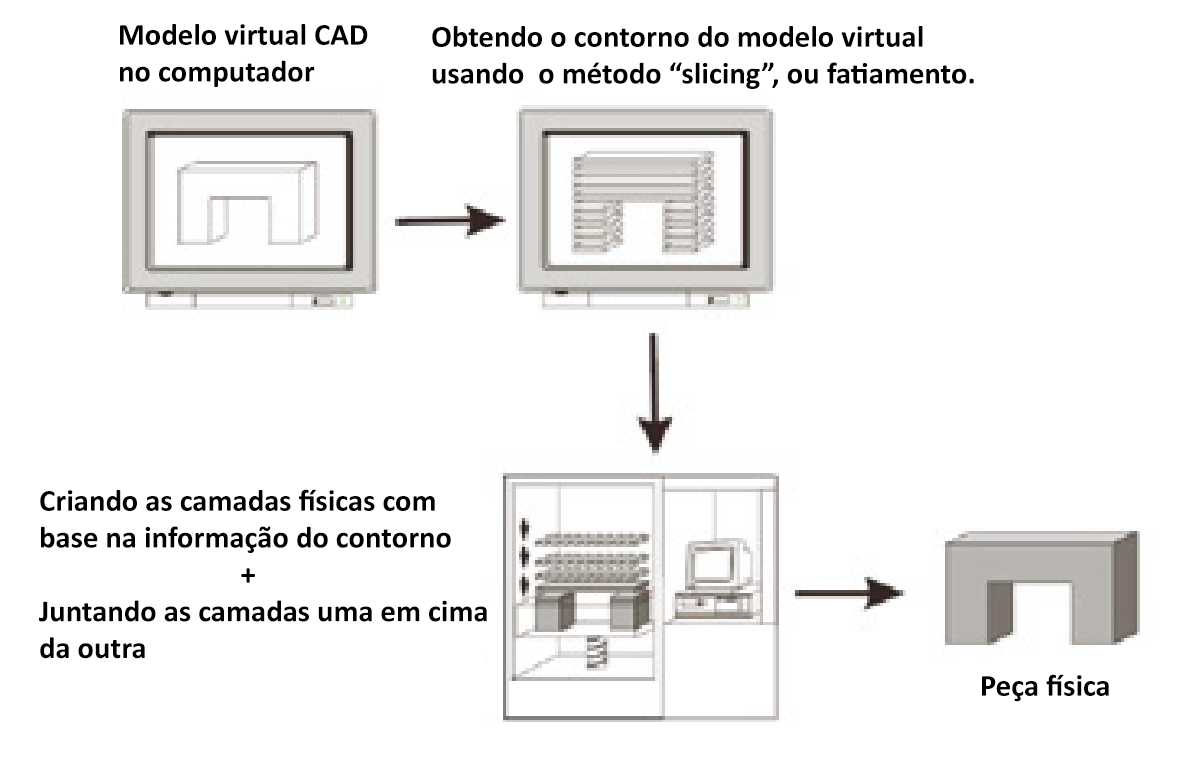
\includegraphics[width=1\textwidth]{figures/manufatura_aditiva}
	\caption{Processo de manufatura aditiva \cite{manufatura_aditiva}}
	\label{fig:manufatura_aditiva}
\end{figure}
